\chapter{MCSA Relaxation Parameters\ }
\label{chap:spn_mcsa_relaxation}
As another means of preconditioning (or variance reduction) to meet
the goal of improving iterative performance, the Richardson iteration
may be implemented with an adjustable scalar relaxation parameter:
\begin{equation}
  \mathbf{x} = \mathbf{x} + \omega \mathbf{r}\:,
  \label{eq:richardson_relaxation}
\end{equation}
where $\omega$ is the relaxation parameter. This is very similar to
point Jacobi preconditioning where the system is now being scaled on
the left by a constant value in all rows. Analogously, these
relaxation parameter techniques can be applied to Monte Carlo to
improve convergence as demonstrated by Dimov \cite{dimov_new_1998}. In
this case, building an iteration matrix from
Eq~(\ref{eq:richardson_relaxation}) gives:
\begin{equation}
  \mathbf{H} = \mathbf{I} - \omega \mathbf{A}\:,
  \label{eq:relaxed_iteration_matrix}
\end{equation}
with the probabilities and weights for the Monte Carlo procedure
appropriately scaled via a modified Neumann-Ulam decomposition. For
MCSA, we can stage this scheme with two separate relaxation
parameters; one for the outer Richardson iteration and one for the
inner Monte Carlo solve:
\begin{subequations}
  \begin{gather}
    \ve{x}^{k+1/2} = \ve{x}^k + \omega_R \ve{r}^k\:,\\ \ve{r}^{k+1/2}
    = \ve{b} -
    \ve{A}\ve{x}^{k+1/2}\:,\\ \omega_N\ve{A}\delta\ve{x}^{k+1/2} =
    \omega_N\ve{r}^{k+1/2}\:,\\ \ve{x}^{k+1} = \ve{x}^{k+1/2} + \delta
    \ve{x}^{k+1/2}\:,\\ \ve{r}^{k+1} = \ve{b} - \ve{A}\ve{x}^{k+1}\:,
  \end{gather}
  \label{eq:mcsa_relaxed}
\end{subequations}
where $\omega_R$ is the Richardson iteration relaxation parameter and
$\omega_N$ is the Neumann-Ulam Monte Carlo solve relaxation parameter.

We apply these relaxation parameters to the fuel assembly problem
defined in \S~\ref{sec:fuel_assembly_calcs} along with the reduced
domain approximation as a means of studying their effects. For each
calculation presented, the number of iterations required to converge
was for a single eigenvalue iteration.  Again, \sn{3}{4} histories are
used at each MCSA iteration to compute the Monte Carlo correction
using the adjoint collision estimator. A reduced domain fill level of
100 is used with a threshold of \sn{1}{-10} to filter small
values. ILUT preconditioning with a drop tolerance of \sn{1}{-5} and
fill level of 5 is used as well.

Figure~\ref{fig:relax_iters} gives the number of iterations required
to converge an eigenvalue iteration of the fuel assembly problem for a
1-group SP1 discretization using varying combinations of the
relaxation parameters. First, both parameters were fixed at the base
case of 1 while the other parameter was varied as shown in the
left-hand side plots of Figure~\ref{fig:relax_iters}. For the
Richardson relaxation parameter, using a value larger than 1 gave
better iterative performance up to a point, effectively providing a
stronger extrapolation using the residual at each iteration. For the
Neumann relaxation parameter, a value of less than 1 is observed to be
ideal. Although initially counter-intuitive, the fact that the
correction computed by the Monte Carlo solver has a stochastic error
associated with it means that by using a Neumann relaxation parameter
less than 1 the correction and its error are effectively dampened to
improve iterative performance.

Considering the CPU time required to converge a single eigenvalue
iteration, similar results are also observed for the relaxation
parameters as given by Figure~\ref{fig:relax_time}. For the base cases
given by the plots on the left, it was found the a Richardson
relaxation parameter of 1.1 and a Neumann relaxation parameter of 0.7
provided the fastest CPU time for convergence. Fixing each parameter
at these new values, the calculations were repeated as shown for the
plots on the right hand sides of both Figures~\ref{fig:relax_iters}
and \ref{fig:relax_time}. For each repeated timing calculation, it was
found that the same combination of relaxation parameters found in the
base cases performed the best although they did not necessarily have
the best iterative performance.

\begin{figure}[t!]
  \begin{center}
    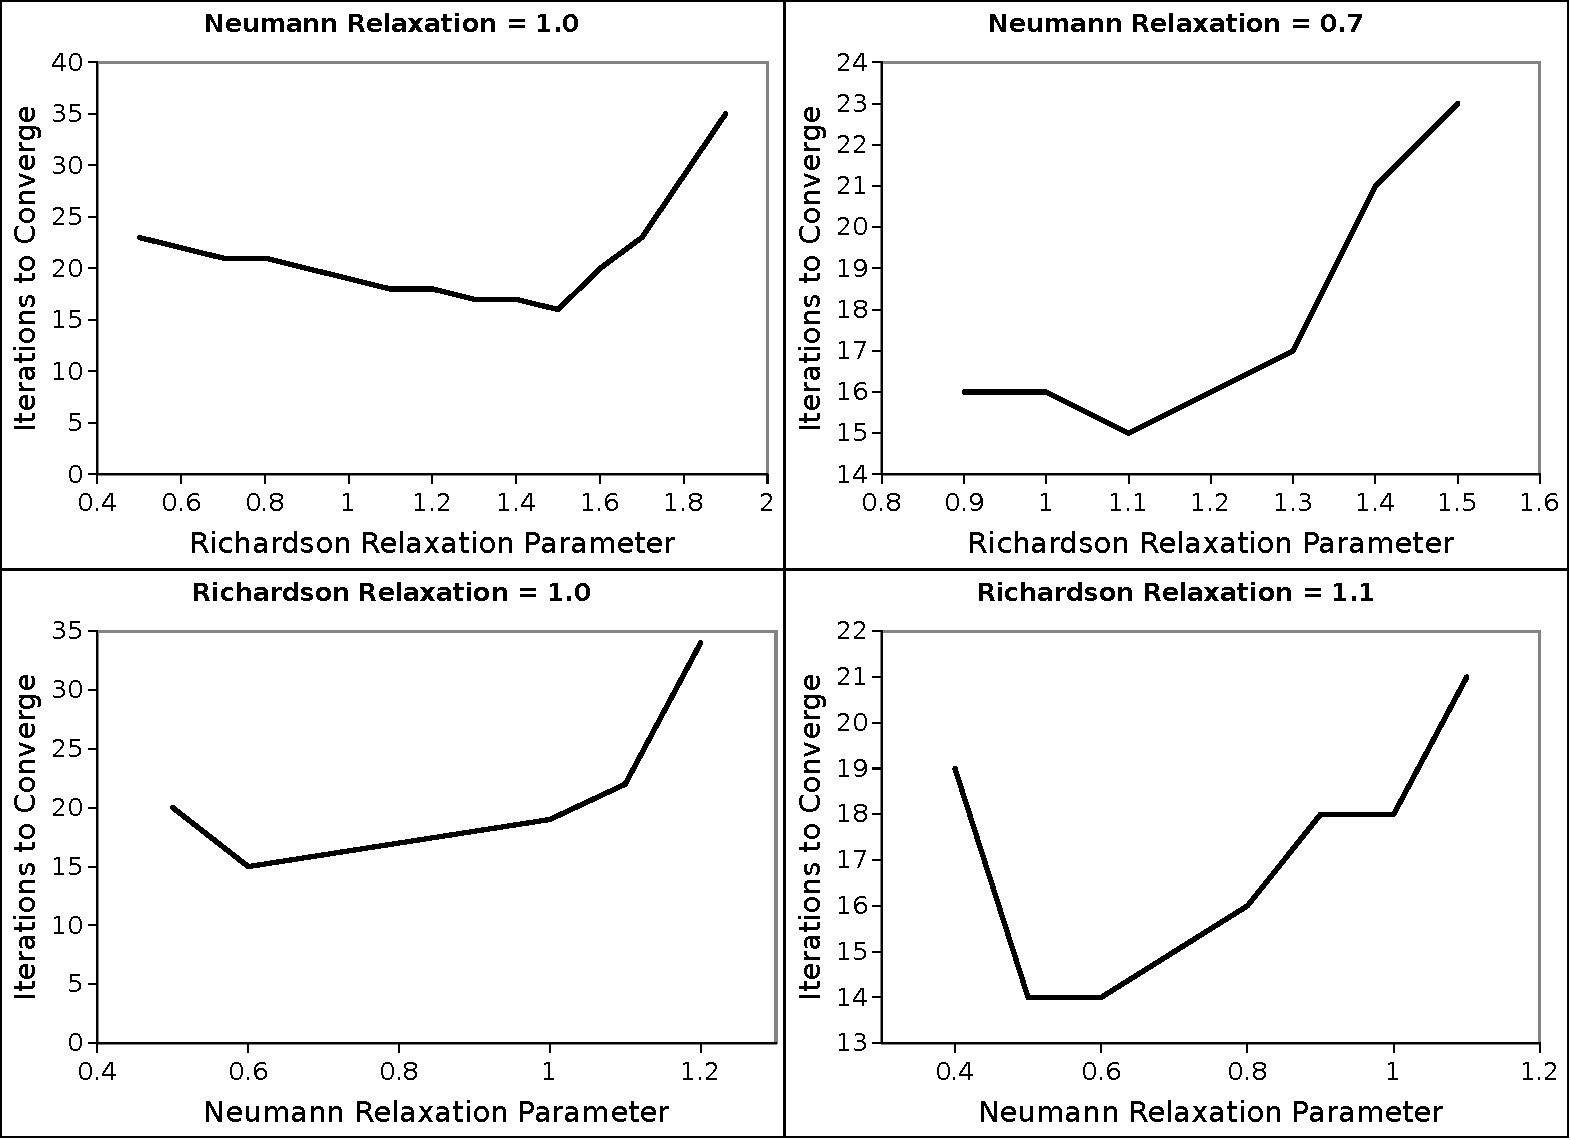
\includegraphics[width=6in]{chapters/spn_equations/relax_iters.pdf}
  \end{center}
  \caption{\textbf{Number of iterations to converge a single
      eigenvalue iteration of the fuel assembly problem as a function
      of the relaxation parameters.} \textit{Starting in upper left
      and moving counter-clockwise: Neumann relaxation parameter fixed
      at 1.0, Richardson relaxation parameter fixed at 1.0, Neumann
      relaxation parameter fixed at 0.7, Richardson relaxation
      parameter fixed at 1.1. For each calculation \sn{3}{4}
      stochastic histories were used to compute the MCSA correction at
      each iteration.}}
  \label{fig:relax_iters}
\end{figure}

\begin{figure}[t!]
  \begin{center}
    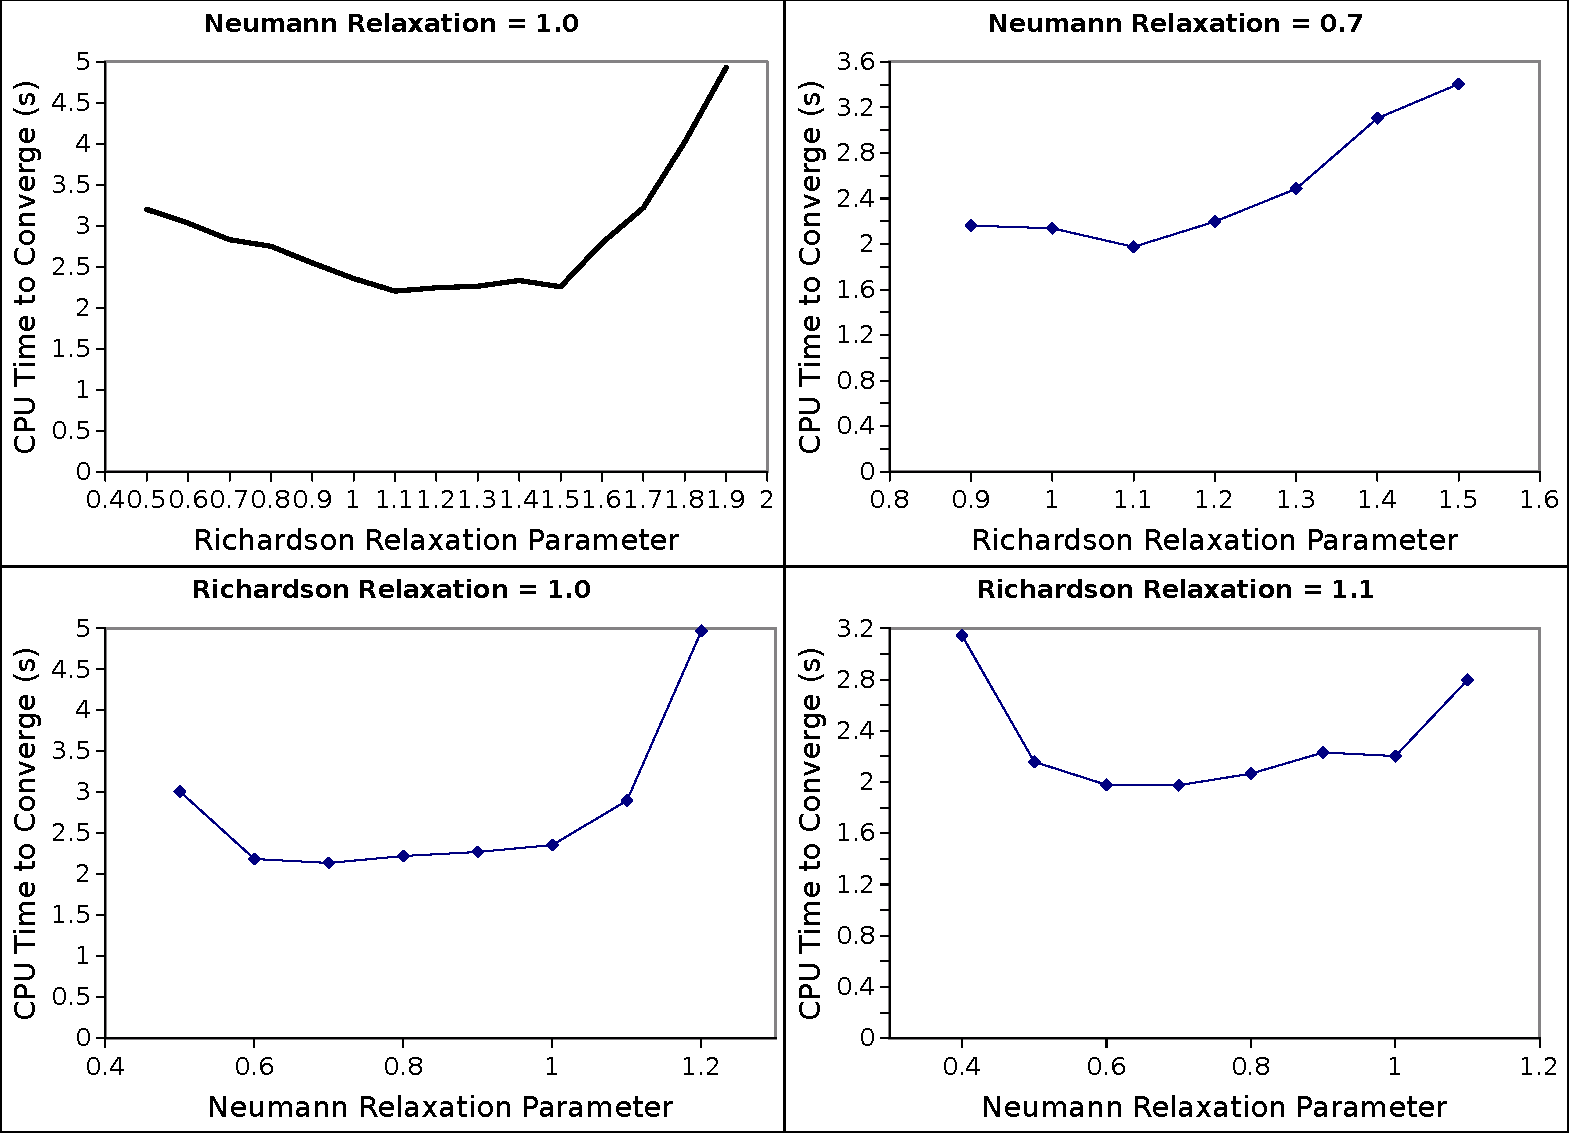
\includegraphics[width=6in]{chapters/spn_equations/relax_time.pdf}
  \end{center}
  \caption{\textbf{CPU time in seconds to converge a single eigenvalue
      iteration of the fuel assembly problem as a function of the
      relaxation parameters.} \textit{Starting in upper left and
      moving counter-clockwise: Neumann relaxation parameter fixed at
      1.0, Richardson relaxation parameter fixed at 1.0, Neumann
      relaxation parameter fixed at 0.7, Richardson relaxation
      parameter fixed at 1.1. For each calculation \sn{3}{4}
      stochastic histories were used to compute the MCSA correction at
      each iteration.}}
  \label{fig:relax_time}
\end{figure}
